El algoritmo que se utilizó para obtener las soluciones es \texttt{Produce-and-Choose}, cuenta con 
dos fases.
En la primer fase se generan cierta cantidad de bundles, e la fase siguiente se seleccionan los 
bundles que serán parte de la solución.\\
A continuación se explican los algoritmos utilizados para cada fase.
\section{Generación de bundles}
El problema de la generación de bundles es NP-hard (agregar ref) por lo que se utilizaron heurísticas para aproximarse a una solución
\subsection{Bundles One-By-One}
La herurística \texttt{BOBO-x} en cada paso se elige un item, denominado pivote, se genera un bundle a partir del pivote. 
El parámetro $x$ define la cantidad de bundles a generar. El caso de que $x$ sea 'Ex' todos los itmes son pivotes.\\
\subsection{Hierarchical clustering}
Para la heurística Hierarchical clustering \texttt{HAC} se define la función de distancia. 
El algoritmo comienza con tantos clusters como cantidad de elementos, cada uno está conformado por un solo ítem y 
en cada paso se unen los dos clusters mas cercanos y que respeten las restricciones.\\
Se realizaron dos variantes con esta solución, cada una con funciones de distancia diferentes. 
Como primera implementación, que llamamos \texttt{SingleHAC}, utilizamos la función $d1(u,v) 
= 1 - s(u, v)$. Ésta función no tiene en cuenta el $\gamma$ para obtener soluciones de bundles más 
diversos o bundles más cohesivos.\\
En cambio para la segunda implementación, \texttt{EfficientHAC} redefinimos la distancia como la 
función $d2(u,v) = 1 - fn\ obj(u,v)$ que tiene en cuenta el $\gamma$ para buscar una mejor 
solución.\\
En la figura ilustramos cuál es la diferencia, al momento de elegir el próximo cluster que debe ser 
fusionado, utilizando las implementaciones \texttt{SingleHAC} y \texttt{EfficientHAC}.
\begin{figure}[H]
  \centering
    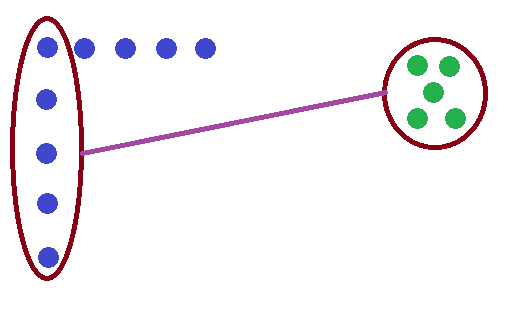
\includegraphics[width=0.3\textwidth]{img/cluster1.png}
  \caption{Selección de bundles usando \texttt{SingleHAC}}
  \label{res:img-usingSingleHAC}
\end{figure}

\begin{figure}[H]
  \centering
    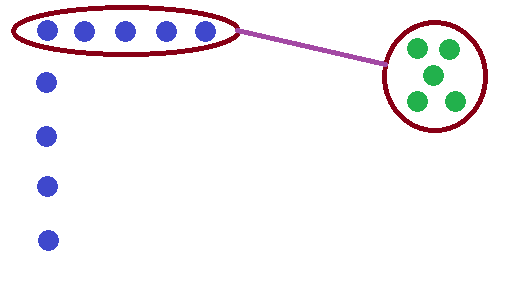
\includegraphics[width=0.3\textwidth]{img/cluster2.png}
  \caption{Selección de bundles usando \texttt{EfficientHAC}}
  \label{res:img-usingEfficientHAC}
\end{figure}

\section{Selección de bundles}
Se utilizaron tres estrategias de selección de bundles para generar las soluciones finales.
\subsection{Selección golosa}
Para la selección de los bundles se utilizó un algoritmo goloso que comienza seleccionando el 
cluster con mayor valor intra y en cada iteración se elige el cluster que maximiza la función 
objetivo.\\
Durante las primeras pruebas notamos que todas las soluciones contenían varios bundles en común 
teniendo en cuenta que se utilizaron distintos valores gammas. Supusimos que esto se debía a que en 
el momento de hacer la selección en todos los casos, sin importar el gamma, se seleccionaba el mismo 
bundle (que es el de mayor intra). Al siguiente paso al seleccionar el bundle que maximiza la 
función objetivo, ocurre que el valor intra del bundle es mucho más significativo que el inter. Por 
lo tanto, lo que ocurre es que en los primeros pasos se seleccionan los mismos bundles para todos 
los gammas sin tener en cuenta que cuando se optó por un gamma cercano a cero se pedía que la 
solución sea más diversificada.\\
\subsection{Selección de a pares}
Para mejorar el proceso de selección se decidió modificar el algoritmo para que en vez de realizar 
la selección de a un bundle, se generan pares de bundles y el algoritmo goloso selecciona el que 
maximiza la función objetivo.
\begin{algorithm}[H]
\begin{algorithmic}[1]
\REQUIRE $produced:Vector<SnowFlake>, numRequested:Integer$
\ENSURE $selected:Vector<SnowFlake>$.
\WHILE {$selected.size < numRequested\ AND\ selected.size < produced.size$}
\STATE $(candidateOne, candidateTwo) \leftarrow (i, j)\ where$ \\ 
$\displaystyle\max_{i \neq j} (fn\ obj(produced_{i},produced_{j})) \wedge isNotUsed(i) \wedge 
isNotUsed(j)$
\STATE $markAsUsed(i)$
\STATE $markAsUsed(j)$
\STATE $selected.push(candidateOne)$
\STATE $selected.push(candidateTwo)$
\ENDWHILE
\RETURN $selected$
\end{algorithmic}
\caption{Selección de bundles de a pares}\label{alg:algSelTuple}
\end{algorithm}
\subsection{Selección proporcional}
Además como tercera opción de selección se implementó un algoritmo proporcional que en cada paso se 
ponderan los resultados de la función que calcula el intra y el inter restante, intentando 
\textquotedblleft adivinar\textquotedblright  el valor de las próximas iteraciones y de esta manera 
dar más importancia en los primeras iteraciones al valor del inter.
\begin{algorithm}[H]
\begin{algorithmic}[1]
\REQUIRE Aca va la entrada del algoritmo.
\ENSURE Aca va la salida del algoritmo.
\WHILE {alguna conodicion}
\STATE Descripcion con palabras.
\IF{alguna conodicion copada}
\RETURN devuelve algo
\ELSE
\STATE alguna asignacion o algo
\ENDIF
\ENDWHILE
\FOR{alguna otra condicion}
\IF{alguna conodicion}
\STATE hace algo
\RETURN devuelve algo
\ENDIF
\ENDFOR
\RETURN devuelve otra cosa
\end{algorithmic}
\caption{Selección de bundles proporcional}\label{alg:algSelProp}
\end{algorithm}

\section{Modificación de PAC para búsquedas específicas}
Para la obtención de la solución se modificó la producción de bundles como así también la 
selección de los mismos (Produce and Choose). \\
En la producción de bundles en el algoritmo jerárquico, se utilizó la similitud del perfil 
específico con los papers en cada paso que intenta unificar dos clusters. A diferencia del cálculo 
original que la compatibilidad de dos nodos esta dada por su distancia previamente obtenida, en 
este nuevo caso se agrega a ese resultado la compatibilidad de cada uno de ellos con el perfil 
específico. \\
Para la producción del algoritmo BOBO, se agregó junto al pivote en todos los clusters. \\
Para la selección de los bundles que formarán parte de la solución, a cada cluster se le 
calculo el valor intra también se tuvo en cuenta la similitud de todos los elementos con el perfil  
específico, de esta manera a los clusters que contenían papers con los mismos tópicos que el del 
vector especifico se le dio mayor peso.

\section{Heurística Golosa}
En todas los algoritmos previos se centraron en, primero construir buenos bundles maximizando solo 
el valor propio de cada bundle, o sea, el valor inter bundle. Una vez generado los suficientes 
\textquotedblleft buenos\textquotedblright  para luego seleccionar dependiendo de la 
estrategia elegida la solución final, ahora si, maximizando la función objetivo propuesta 
originalmente.\\
Para este heurística golosa propusimos ir construyendo los bundles finales teniendo en cuenta en 
cada paso la función objetivo, esto es, en cada paso cuando se intenta agregar un nuevo elemento a 
un bundle se calcula su valor total de la función y se evalúa en que bundle conviene agregarlo. 
Esto se repite para todos los items, haciendo que cuando tengo que agregar un nuevo ítem a la 
solución ya calculé para todos los items que no se encuentran en la solución en que bundle conviene 
agregarlo y cual es el valor de la función en ese caso, quedándonos siempre con el mejor valor 
posible.
\begin{algorithm}[H]
\begin{algorithmic}[1]
\REQUIRE Aca va la entrada del algoritmo.
\ENSURE Aca va la salida del algoritmo.
\WHILE {alguna conodicion}
\STATE Descripcion con palabras.
\IF{alguna conodicion copada}
\RETURN devuelve algo
\ELSE
\STATE alguna asignacion o algo
\ENDIF
\ENDWHILE
\FOR{alguna otra condicion}
\IF{alguna conodicion}
\STATE hace algo
\RETURN devuelve algo
\ENDIF
\ENDFOR
\RETURN devuelve otra cosa
\end{algorithmic}
\caption{Algoritmo heurística golosa}\label{alg:algHeuGol}
\end{algorithm}
